%; whizzy paragraph -pdf xpdf -latex ./whizzypdfptex.sh
%; whizzy-paragraph "^\\\\begin{frame}"
% latex beamer presentation.
% platex, latex-beamer でコンパイルすることを想定。 

%     Tokyo Debian Meeting resources
%     Copyright (C) 2008 Junichi Uekawa

%     This program is free software; you can redistribute it and/or modify
%     it under the terms of the GNU General Public License as published by
%     the Free Software Foundation; either version 2 of the License, or
%     (at your option) any later version.

%     This program is distributed in the hope that it will be useful,
%     but WITHOUT ANY WARRANTY; without even the implied warranty of
%     MERCHANTABILITY or FITNESS FOR A PARTICULAR PURPOSE.  See the
%     GNU General Public License for more details.

%     You should have received a copy of the GNU General Public License
%     along with this program; if not, write to the Free Software
%     Foundation, Inc., 51 Franklin St, Fifth Floor, Boston, MA  02110-1301 USA

\documentclass[cjk,dvipdfmx,12pt]{beamer}
\usetheme{Tokyo}
\usepackage{monthlypresentation}

%  preview (shell-command (concat "evince " (replace-regexp-in-string "tex$" "pdf"(buffer-file-name)) "&"))
%  presentation (shell-command (concat "xpdf -fullscreen " (replace-regexp-in-string "tex$" "pdf"(buffer-file-name)) "&"))
%  presentation (shell-command (concat "evince " (replace-regexp-in-string "tex$" "pdf"(buffer-file-name)) "&"))

%http://www.naney.org/diki/dk/hyperref.html
%日本語EUC系環境の時
\AtBeginDvi{\special{pdf:tounicode EUC-UCS2}}
%シフトJIS系環境の時
%\AtBeginDvi{\special{pdf:tounicode 90ms-RKSJ-UCS2}}

\title{東京エリア Debian 勉強会}
\subtitle{資料}
\author{上川 純一 dancer@debian.or.jp\\IRC nick: dancerj}
\date{2008年12月20日}
\logo{
\includegraphics[width=8cm]{image200607/openlogo-light.eps}}

\begin{document}

\frame{\titlepage{}}

\emtext{設営準備にご協力ください}

\section{}
\begin{frame}
 \frametitle{Agenda}
\begin{minipage}[t]{0.45\hsize}
  \begin{itemize}
  \item 注意事項
	\begin{itemize}
	 \item \underline{飲食禁止}
	 \item 政治/宗教/営利活動禁止
	 \item ustream にて試験ストリーミング中
	\end{itemize}
  \item 最近のDebian関連のイベント
	\begin{itemize}
	 \item 前回の勉強会
	\end{itemize}
 \end{itemize}
\end{minipage} 
\begin{minipage}[t]{0.45\hsize}
 \begin{itemize}
  \item Debianの2008年をふりかえり、2009年を予想する
  \item ライトニングトーク
 \end{itemize}
\end{minipage}
\end{frame}

\section{最近}

\begin{frame}
 \frametitle{11月}
\begin{minipage}[t]{0.45\hsize}
  \begin{itemize}
  \item 注意事項
	\begin{itemize}
	 \item 飲食禁止
	 \item 政治/宗教/営利活動禁止
	 \item ustream にて試験ストリーミング中
	\end{itemize}
  \item 最近のDebian関連のイベント
	\begin{itemize}
	 \item 前回の勉強会、Debconf
	\end{itemize}
 \end{itemize}
\end{minipage} 
\begin{minipage}[t]{0.45\hsize}
 \begin{itemize}
  \item 「その場で勉強会資料を作成しちゃえ」 Debian を使った LaTeX 原稿作成合宿
 \end{itemize}
\end{minipage}
\end{frame}


\section{DWN quiz}
\begin{frame}{Debian 常識クイズ}

Debian の常識、もちろん知ってますよね?
知らないなんて恥ずかしくて、知らないとは言えないあんなことやこんなこと、
みんなで確認してみましょう。

今回の出題範囲は\url{debian-devel-announce@lists.debian.org} に投稿された
内容とDebian Project Newsからです。

\end{frame}

\subsection{問題}

% TODO: fill here.

\section{最近のDebian関連のイベント}


\section{事前課題紹介}
\emtext{事前課題の紹介}
% pre work home work

\begin{frame}{事前課題}

今回の事前課題は
前回の演習を踏まえて \LaTeX{}で作成していただきました。
トピックは以下の二つのうち一つを選択することになっていました。

\begin{enumerate}
 \item Debian勉強会で今年やったこと、来年したいこと
 \item \LaTeX{}+Gitの事前課題ができなかった、こんなハマり方しました体験記
\end{enumerate}

\end{frame}

% (query-replace "\\subsection" "\\end{frame}\\begin{frame}")
% (query-replace "\\subsubsection" "\\textbf")

{\footnotesize
%; whizzy-master ../debianmeetingresume200812-presentation.tex
%%; whizzy-master ../debianmeetingresume200812.tex

\begin{prework}{������}

��ǯ��ä���ǯ��ꤿ�����Ȥ�ͤ��Ƥߤޤ�����

\preworksection{��ǯ��ä�����}

\begin{itemize}
 \item ��ǯ�κǽ�˷ײ�򤿤ƤƤߤ����ǽ�Ū�ˤϤ��Τޤ޼»ܤϤ��ʤ��ä�
       ���ɡ��ʤ�餫�Υ����ǥ��θ����ˤϤʤä���
 \item \LaTeX{} �Υϥ󥺥�����ä���
 \item Debian �ѥå����������Τ���ΰ�Ϣ�ιֺ¤��äƤߤơ�
       �������ֻ���򤤤������ʿͤ����ˤ��Ƥ��ä���
\end{itemize}
�Ȥ����Τ�����ޤ�����

\preworksection{��ǯ��ꤿ���ʤ��ȻפäƤ���Τ�}

���������ȥϥ󥺥���Ū�ʤ�Τ����䤷�Ƥ���������

\begin{itemize}
 \item DocBook�Υϥ󥺥���
 \item �ѥå����������Υϥ󥺥���
 \item avahi �γ��ѹֺ�
 \item \LaTeX{}��Ϣ�Τ������ΥХ���ľ����
 \item screencast / �ӥǥ�����ե���� / ���ȥ꡼�ߥ󥰴�Ϣ�β���
\end{itemize}
�������ͤ��Ƥ��ޤ���

\end{prework}

\begin{prework}{ʿ߷�ӷ�}

\preworksection{Debian�ٶ����ǯ��ä����ȡ���ǯ����������}
�����3���λ��äǤ���
�ǥӥ���⤽���Ǥ���������ʤ����Ȥ��餱�ʤΤǡ�
��ǯ�ϳ��оޤ�ͤ餤�Ĥġ������ȤǤ���褦�ˤʤ�Ȥ����ʤ�

\preworksection{\LaTeX{}+Git�λ������꤬�Ǥ��ʤ��ä�������ʥϥޤ������ޤ����θ�
       ��}
\LaTeX{}�Ϥޤ������Ĥ����ʤ�Ƥ������ʤΤǥ��ȥ쥹̵�Ǥ�����
�ӥ�vi�ʤ錄���ˤ�emacs���ʤ�Ȥ⤤�������Ϥ�����
�äƤ��󤸤ǤȤƤ��ϫ���Ƥ��ޤ���
���������ʸ�Ϥ������Τ�10ʬ���餤�����äƤ����Ǥ���

���������β�����̤��Ƥޤ��褯�狼�äƤ��ʤ��ʤ���
������Ȥ�����
\begin{itemize}
 \item git������
 \item ����ޥ����ʤ��Ȥ���santaku�Ȥ�)
 \item �����Ƥ����ޤä���
\end{itemize}

����ʤ�ΤǴ��ۤ��Ƥ�������

\end{prework}
\begin{prework}{ƣ������}

\preworksection{��Debian�ٶ���Ǻ�ǯ��ä����ȡ���ǯ���������ȡ�}

��ǯ�ϡ�3��ޤǤϴ���Debian�ٶ���4����������ꥢDebian�ٶ���˻���
���ޤ����ʲ��٤��������塼����Թ�ǻ��äǤ��ޤ���Ǥ������ˡ�
����ܿ������μ��˿������Ȥ������ǡ��ٶ���Ȥ�����ϼ�ʬ�ˤȤä�̥��
Ū�ʤ�ΤǤ��������٤Ƥ���٤˵ۼ�����Τ��񤷤����Ȥ�ƨ������Τ⤢���
���������������λ���������뤳�Ȥ����꤬�����Ǥ���

��Ū�˺�ǯ��ȿ�ʤȤ��ơ�
\begin{itemize}
\item �ٶ���ǰ���줿���Ƥ��Ф��ơ���ʬ��try and error�λ��֤���ݤǤ�
      �ʤ��ä�
\item �ٶ����Debian Project���Ф��Ʋ���׸����Ƥ��ʤ�
\end{itemize}
�Ȥ���2������ǯ�ϲ������Ƥ��������ȹͤ��Ƥ��ޤ���

\preworksection{��ǯ��}

�嵭��Ƨ�ޤ��� \textbf{��1�桼�������æ�ѡ�}���ܻؤ��ƴ�ĥ����
�Ȼפ��ޤ������Τ���ˤޤ���
\url{http://www.debian.or.jp/community/devel/}�˽񤤤Ƥ��뤳�Ȥ�ǯ��ǯ��
�����Ѥ������򤷤Ƥ��������Ȼפ�����Ǥ���

\end{prework}
\begin{prework}{���Ĺ�ʿ}
\preworksection{Debian �ٶ���Ǻ�ǯ��ä����ȡ�}

��ǯ�ϡ��ѥå������κ�����ȯɽ��Ԥ��ޤ������������ä����ĥå��ߤ򤤤���
��ĺ�����Τˡ������������Ƥ��ʤ��ä����Ȥ������Ȥ˺����ʤ��鵤�Ť��ޤ�
������������Ǥ��͡�
���Ȥϡ�Debian �� ``��''�Ͻв񤤷Ϥ�``��''�˹׸��������ȡ��ʤ��

\preworksection{��ǯ�ؤη��ɽ����}
\begin{itemize}
 \item �ͥ���ȯɽ���ٶ���α��Ĥˤ�ä��Ѷ�Ū�˻��褷�Ƥ����ޤ�������ʤ��ơ�\textbf{``����
��''}��
 \item Debian �ٶ���ؤλ��üԡ�Debian �γ�ȯ�Ԥ����䤹�������ˡ��ͤ�
       �ޤ���
 \item ���� Debian �桼���ˤ��ơ��ٶ����Ϣ��Ƥ��ޤ���
\end{itemize}

\end{prework}
\begin{prework}{���Ĥ���}

\preworksection{��Debian�ٶ���Ǻ�ǯ��ä����ȡ�}

�ٶ���˻��ä��ơ�

\begin{itemize}
 \item �ѥå�����������Ϣ(OSC�ǤΥϥ󥺥���ޤ�)
 \item \LaTeX{}�ϥ󥺥���
\end{itemize}
���ٶ��ˤʤä���
�ʤ�Ȥʤ��ѥå����������Ǥ���褦�ˤʤäƤ����Τǡ��⤦���ʥ��ƥåץ��å�
��������

\preworksection{��Debian�ٶ������ǯ���������ȡ�}

��ɸ�Ȥ��Ƥϡ�
\begin{itemize}
 \item �ٶ���λ��ò�������䤹
 \item �����η����ٶ���Debian Project�˹׸�������
\end{itemize}

�ٶ���Υͥ��Ȥ��Ƥϡ�
\begin{itemize}
 \item �ѥå���������
 \item �Х���ݡ��ȥϥ󥺥���
 \item �絬�ϤʴĶ��ǤΡ�Debian�����д�����ˡ���ѥå������ΰ���Ŭ�ѤȤ�
       ����ե�����δ����Ȥ����ºݱ��Ѥ��Ƥ��������ä�ʹ���Ƥߤ����Ǥ���
\end{itemize}
�Ȥ��ä������Ǥ��礦����

\end{prework}
\begin{prework}{��ޤ�������}

\textbf{Debian�ٶ���Ǻ�ǯ��ä����ȡ���ǯ����������}

�ٶ���ˤ�11��黲�ä��Ϥ᤿�Ф���� Debian �鿴�ԤʤΤǡ���ǯ��ä����Ȥ�
��ǰ�ʤ����Ĥ����ʤ��ΤǤ���...

\textbf{��ǯ��ä�����}

\begin{itemize}
\item avahi �ν����λؼ�����Ȥ��Ƥ����Τǡ������� DHCP server ����
      �����������ˤ���ޤ���(Windows �� VMware ��� Debian ��ư�����Ƥ�������)
\item \TeX ��������
\end{itemize}

\preworksection{��ǯ����������}

\begin{itemize}
 \item git �Υϥ󥺥���
 \item �ѥå����������Υϥ󥺥���
 \item �����Υϥ󥺥���
\end{itemize}
�����꤬�Ǥ���Ȥ����ʤ��ȻפäƤ��ޤ���

\end{prework}
\begin{prework}{���� ʸ}
\begin{itemize}
\item Debian�ٶ���Ǻ�ǯ��ä�����\\
��ǯ���ؤ���ٶ���ϻ��ä��ޤ���Ǥ�����������
�Ȥꤢ���������DD�ϻ��ߤޤ�����

\item  ��ǯ����������\\
����Ū�ʻ��Ǥ���,��ä�C��kernel���ٶ�������Ǥ���
���server��Tuning���äȽ����褦�ˤʤꤿ����
����Ȼ��������οͤ�õ�����������ǥޥޤǥ����ƥ��äƤ���ͤ��ʤ����ʤ�������

 \item \LaTeX{}+Git�Ǥ���ʥϥޤ������ޤ����θ���\\
anthy+scim�����Ϥ����ƤʤΤǤ��ʤ���֤�������ޤ�����
\end{itemize}

\end{prework}
\begin{prework}{���� ����}

\preworksection{Debian�ٶ���Ǻ�ǯ��ä�����}
��ǯ�ϡ�debhelper+CDBS+quilt/dpatch�ǤΥѥå������󥰤˴ؤ����äȡ�
Po4a���Ѥ����������ƥʥ󥹤ˤĤ��Ƥ��ä򤷤ޤ�����

\preworksection{Debian�ٶ������ǯ����������}
��ǯ�ϡ�buildd���Ѥ�����ư�ӥ�ɤˤĤ����ä��Ǥ�����Ȼפ��ޤ���
�ޤ�������äȼ��ư�����ƤߤƤ��뤳�Ȥ������Ĥ�����Τǡ�
������⤦����������Ȥ����������ˤ���ȯɽ�������Ǥ���

�Ǹ�ˡ���ǯ������Debian Developer�ˤʤꤿ���Ǥ���

\end{prework}
\begin{prework}{�����ϥ�}
\begin{itemize}
\item Debian�ٶ���Ǻ�ǯ��ä�����\\
���פ������פϷ򹯾����ͳ�ǡ����ޤ껲�äǤ��ޤ���Ǥ����ͤ���
���פǤϡ���ǯstable���ѼԤˤ⤫����餺sid��Ƴ�������ꡢ
��ǯ�֤��TeX�����ä��ꡢ�����Ÿ���ˤʤäƤ��ޤ����ʺ��⡦������

\item  ��ǯ����������\\
�ٶ���λ������꤬������ʹߤ⤳�η����ˤʤ�ʤ�С�emacs��Ф��ʤ���
�����ʤ��Τ��ʤ���������Ū��*nix�Ķ��Ǥϡ�vi�ɤʤΤǤ�����
�ʡ������ȸ�����ꡢemacs�ޤä����Ȥ��ޤ��󡪡�
\end{itemize}

\end{prework}
\begin{prework}{���ܡ���Ƿ}
��ǯ�⤢�ޤ��礷�����Ȥ�ʤ����˲᤮��äƤ��ޤ��ޤ�����

\textbf{��ǯ��ä�����}
\begin{itemize}
\item �Ρ��侾���󤬹ֱ餷�� live-helper �λȤ������������OSC �ˤ� Live
      DVD �����ۤ��ޤ�����
\item ���Ӥ���ιֱ�˿�ȯ���졢CDBS �ˤƥѥå���������ޤ�����
\end{itemize}

\textbf{��ǯ����������}
\begin{itemize}
\item �Ѹ���ٶ����������ط� (���ɤȤ�) �Ǥ�׸���������
\item emacs ���äȤ��ޤ��Ȥ���褦�ˤʤꤿ���Ǥ� (��)
\end{itemize}

\end{prework}
\begin{prework}{�侾 ����}
\preworksection{��ǯ}

��ǯ�ϰʲ��Τ褦�ʤ��Ȥ�Ԥ��ޤ�����
\begin{itemize}
 \item Debian�ѥå������󥰥ϥ󥺥�����ä���
 \item Git �ˤɤäפ�ȤĤ��ä���
 \item git-buildpackage / VCS �� Debian�ѥå������ˤĤ��ƹͤ��Ƥߤ���
 \item �����ͥ�¦����Υѥå������˴ؤ��륢�ץ������򤷤Ƥߤ���\\
   Linux kernel patch / kernel module �ˤĤ����ä�����
 \item ��ɤ��ä���
 \item Ustream ��Ȥä����ȥ꡼�ߥ󥰤�Ԥä���
 \item ����������ؤ�ĩ��(Perl/Ruby/Lua)��������ؤλ��ä�Ԥä���
 \item ¾���ٶ���ȤΥ���ܤ򤷤���
 \item �ٶ��񱿱Ĥ�Ԥä���
 \item ���ݡ��Ȥ���ѥå����������䤷����
\end{itemize}

\preworksection{��ǯ����ɸ}

\begin{itemize}
 \item DD�ˤʤ�
 \item SH �ݡ��ƥ��󥰡�wanna-build/buuildd �ط�
 \item ��̥쥤������Ȥθ�ή
 \item �ӥǥ��ط������ȥ꡼�ߥ󥰤Υ��ݡ��ȶ���
 \item �����ͥ�ط��Ǥ� Debian�ؤι׸�
\end{itemize}

\end{prework}

}

\emtext{2008年計画}

\begin{frame}{2008年計画}

{\scriptsize
\begin{enumerate}
 \item 新年会「気合を入れる」
 \item Open Source Conference Tokyo (3/1)
 \item データだけのパッケージを作成してみる、
       ライセンスの考え方 (David Smith)
 \item バイナリ一つのパッケージを作成してみる (吉田@板橋)\\
       バージョン管理ツールを使いDebianパッケージを管理する(git)\\
       アップストリームの扱い(svn/git/cvs)(岩松 信洋さん)
 \item バイナリの分けたパッケージの作成。(前田さん)\\
       バイナリの分け方の考え方、アップグレードなどの運用とか。
 \item パッケージ作成(dpatch/debhelperで作成するパッケージ)(小林儀匡さん)\\
       man の書き方(roff or docbook)(でんさん)\\
       Open Source Conference Hokkaido
 \item パッケージ作成(kernel patch、kernel module)
       、Debconf発表練習
 \item Debconf アルゼンチン、Debian温泉

 \item Open Source Conference Tokyo/Fall、
       デーモン系のパッケージの作成、\LaTeX{}、 emacs-lisp、フォントパッケージ
 \item パッケージの cross-compile の方法、amd64 上で i386 のパッケージと
       か、OSC-Fall報告会、Debconf報告会
 \item 国際化 po-debconf / po化 / DDTP
 \item 忘年会
\end{enumerate}
}
\end{frame}

\begin{frame}{2008年実績}

{\scriptsize
\begin{enumerate}
 \item 新年会「気合を入れる」
 \item Open Source Conference Tokyo (3/1)
 \item データだけのパッケージを作成してみる、
       ライセンスの考え方 (David Smith)
 \item バイナリ一つのパッケージを作成してみる (吉田@板橋)\\
       バージョン管理ツールを使いDebianパッケージを管理する(git)
       $\rightarrow$  なし\\
       アップストリームの扱い(svn/git/cvs)(岩松 信洋さん)
       $\rightarrow$  なし
 \item バイナリの分けたパッケージの作成。(前田さん)\\
       バイナリの分け方の考え方、アップグレードなどの運用とか。       $\rightarrow$  なし
 \item パッケージ作成(dpatch/debhelperで作成するパッケージ)(小林儀匡さん)\\
       man の書き方(roff or docbook)(でんさん) $\rightarrow$  なし\\
       Open Source Conference Hokkaido $\rightarrow$  なし
 \item パッケージ作成(kernel patch、kernel module)\\
       Debconf発表練習 $\rightarrow$  なし
 \item Debconf アルゼンチン、Debian温泉
 \item Open Source Conference Tokyo/Fall\\
       デーモン系のパッケージの作成、\LaTeX{}、 emacs-lisp、フォントパッケージ
       $\rightarrow$  なし
 \item パッケージの cross-compile の方法、amd64 上で i386 のパッケージと
       か、OSC-Fall報告会、Debconf報告会  $\rightarrow$  なし
 \item 国際化 po-debconf / po化 / DDTP  $\rightarrow$  なし
 \item 忘年会
\end{enumerate}
}
\end{frame}

\emtext{2008年の振り返り}

\section{}
\begin{frame}{東京エリアDebian勉強会の参加者の推移}
 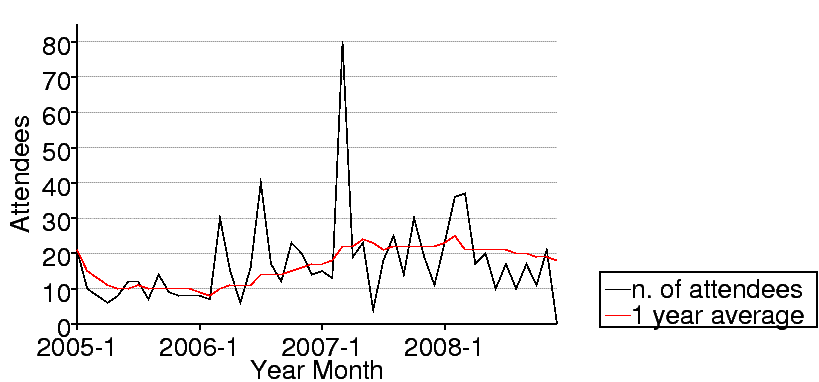
\includegraphics[width=1\hsize]{image200812/serialized.png}
\end{frame}

\begin{frame}{参考: 関西Debian勉強会の参加者の推移}
 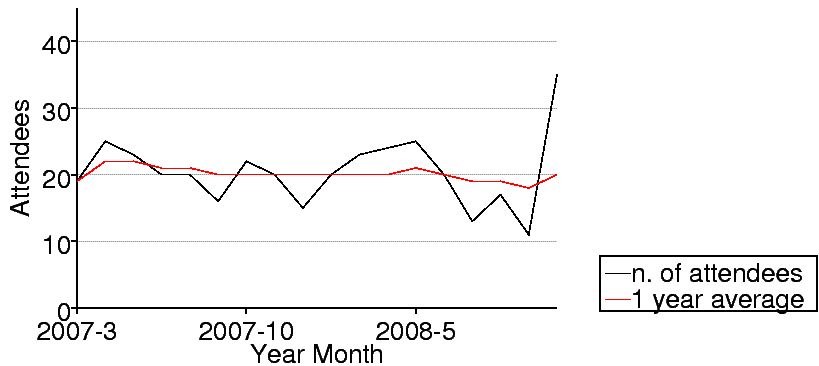
\includegraphics[width=1\hsize]{image200812/kansai.png}
\end{frame}

\begin{frame}{東京エリアDebian勉強会の事前課題・事後課題の推移}
 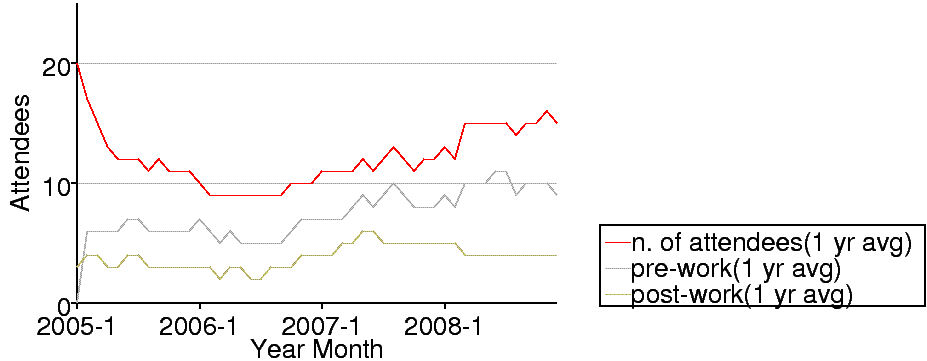
\includegraphics[width=1\hsize]{image200812/memberanalysis/attend.png}
\end{frame}

\emtext{2009年を計画する}

\begin{frame}{タイムライン}

{\scriptsize
\begin{tabular}[t]{|p{2em}|p{3em}|p{9em}|p{7em}|p{6em}|}
\hline
2006 &2007 &2008 &2009 & 2010 \\
\hline
%2006
IntelMacに、coreduoでdual-core CPU に、 

glantank(ARM)、 
OpenMicroServer(MIPS)、 

OpenSolarisが出てDebian/Solaris (Nexenta) 登場、 
SparcT1がオープンに、

CC3.0、

Qwik登場(?)、

雑誌が大多数消失、

 &
%2007
VT・AMD-V(仮想化技術)が普及(ML115!)、

黒箱(ARM)、
OpenBlocks(PPC?)、
iPhone登場、 
HSDPA 月額5000円くらいに、
google mobile、

VISTAリリース、 
Leopardリリース、 

GPL3.0、
メモリ2Gがコモディティーに、
SparcT2がオープン、 
ニコニコ動画、
& 
%2008
python 3.0
ruby 1.9

wine 1.0, wine64 登場

RoR 2.0 登場で普及に

4コア・64bit のCPUがデスクトップに普及、
Core2Quad 値下げ。

ニコニコ動画1000万ユーザ突破、
初音ミクブームに

地デジ関連のPC製品の普及

勉強会の普及(楽天とか)

公衆無線LAN (wireless gate)

携帯電話の売上が落ちる、
iPhone, Android 登場、
emobile 100円PC抱きあわせ
(eeePC, Dell mini9)
Zaurus販売終了。

Chumby 発売。

サーバの仮想化 ESXi・シンクライアント

MacBook Air 発売、
無線 802.11n が実機に

SystemZ10 発表

世界経済の崩壊(IT投資緊縮財政、職を失う人が増加)

FreeBSD 7 (malloc, ZFS ?)

Debian次世代育成計画始動

Debian Maintainer 制度始動

セキュリティー関連(OpenSSL 事件、DNS事件)

クラウド関連が流行?

Nintendo DSi

&
%2009

tile window manager boom ?

Lenny リリース予定

Debian 合同結婚式

デスクトップ、8コア、4GB? 8GB?

ノートパソコン、2コア、2GB?

Linux が標準インストールのPC。

SSD の値段と容量がこなれる?
HDDがなくなる?高くなる?

ファイルシステムかわる?

ipv6 使えるようになってる?

Bluray が普及?

DL禁止法? torrent に逆風?

&
%2010

消費税上昇に伴う繁忙期

クラウドにより、単純なホスティング業者がつづかない?
一部は自社でもつようになる?

Squeezeリリース

USB 3.0 搭載、wireless USB vs Bluetooth ?

組み込みCPUはAtomに統一?Armは残ってる?

kFreeBSD オフィシャルアーキテクチャに

ruby 2.0 リリース?


\\

\hline
\end{tabular}

}
\end{frame}

\begin{frame}{SWOT}

%SWOT
{\tiny
\begin{tabular}[t]{|p{8em}|p{8em}|p{8em}|p{8em}|}
\hline
できたこと & できなかったこと & チャンスとなるもの & 脅
 威となるもの \\
\hline
%S 
嫁ができた。(20\%、10\% 2次元)
将来のDDが生まれた。

Hands-on(パッケージ作成と\LaTeX{}) と合宿(温泉とブレスト)、
DMCができた。

持ち回りで発表する

場所がいろいろだった。(上川不在)

他の勉強会(カーネル読書会)に殴り込み(岩松、山根)

Ubuntuとの交流、Debian JPに寄付



&
%W

当初の目標であった女子高生、大学生への勧誘が成功しなかった。

嫁ができなかった(70\%、想像力がたりない)

発表やりたかったけどできなかった(でんさん)

GNU/Hurd、SuperH

Debconfにいけなかった(上川以外)

日本へのDebconf招致活動未完

&
%O
	 
所帯持ちハック方法が生まれる(いかにして時間をつくるか)。

無駄な買い物をしなくなる。
ハックしないと。

東京オリンピックの成立?

学生の就職率低下、大学院生増加?ニート増加?

GPLv3 の普及?
Android?

&
%T

環境整備ができなくなる(
ボーナスが減った、
仕事がなくなるかも)

Atom によるCPUアーキテクチャーの駆逐

ハックできないデバイスの増加(電話とか)

法制度の強化により自由がうばわれる?

従量制課金に移行?

\\
\hline
\end{tabular}
}
\end{frame}
\subsection{SWOT 2}

\begin{frame}{SWOT 2}

% SWOT 2
{\tiny

\begin{tabular}[t]{|p{1em}|p{16em}|p{12em}|p{12em}|}
\hline
 &  & チャンスとなるもの & 脅威となるもの  \\\hline

 & & 
%O
	 
所帯持ちハック方法が生まれる(いかにして時間をつくるか)。

無駄な買い物をしなくなる。
ハックしないと。

東京オリンピックの成立?

学生の就職率低下、大学院生増加?ニート増加?

GPLv3 の普及?
Android?

&
%T

環境整備ができなくなる(
ボーナスが減った、
仕事がなくなるかも)

Atom によるCPUアーキテクチャーの駆逐

ハックできないデバイスの増加(電話とか)

法制度の強化により自由がうばわれる?

従量制課金に移行?

\\
\hline
できたこと & 
%S

嫁ができた。(20\%、10\% 2次元)
将来のDDが生まれた。

Hands-on(パッケージ作成と\LaTeX{}) と合宿(温泉とブレスト)、
DMCができた。

持ち回りで発表する

場所がいろいろだった。(上川不在)

他の勉強会(カーネル読書会)に殴り込み(岩松、山根)

Ubuntuとの交流、Debian JPに寄付

&

東京オリンピックの会場でハック。

学校にお願いして学生を勧誘する・ハンズオン。

「君のさわっているXXはLinuxだけどより詳しく知りませんか?」
(ミニノートのプリインストール、携帯、Android)

& 

よりよいネットワークプロトコルを実施

アンチAtom?

\\
\hline

できなかったこと
&
%W

当初の目標であった女子高生、大学生への勧誘が成功しなかった。

嫁ができなかった(70\%、想像力がたりない)

発表やりたかったけどできなかった(でんさん)

GNU/Hurd、SuperH

Debconfにいけなかった(上川以外)

日本へのDebconf招致活動未完

&

Debconf にいく。

時間をつくる、ライフハック(所帯持ちハック)。

専門学校、工業高校、大学での開催。


言語系のコミュニティーに切り込む

インフラ系の人たちに切り込む

非常勤講師になる。

&

\\
\hline
\end{tabular}
}
\end{frame}

\emtext{LT}

\begin{frame}{LT}

 \begin{itemize}
  \item 小林さん
  \item  id774
  \item 上川
  \item やまださん
  \item 岩松
  \item 前田さん
  \item 日比野さん
 \end{itemize}
 
\end{frame}

\emtext{sqlite3をつかってみた}
\section{sqlite3}
\begin{frame}{はじめに: sqlite3 とは?}

 お手軽なSQLデータベース

 \fbox{\includegraphics[width=1\hsize]{image200812/sqlite.eps}}
\end{frame}

\begin{frame}[containsverbatim]{インストール}

\begin{commandline}
# apt-get install sqlite3 python-pysqlite2
\end{commandline}

以上。

%$
\end{frame}

\begin{frame}[containsverbatim]{簡単:データベースの作成}

データベースを作成してみる!

\begin{commandline}
$ sqlite3 debmtg.db
sqlite> 
\end{commandline}
%$
\end{frame}


\begin{frame}[containsverbatim]{独自だけど簡単なインタフェース}
\begin{commandline}
$ sqlite3 /tmp/a.db 
SQLite version 3.5.9
Enter ".help" for instructions
sqlite> create table unko(test text, count number); 
sqlite> .tables
unko
sqlite> .dump unko
BEGIN TRANSACTION;
CREATE TABLE unko(test text, count number);
COMMIT;
\end{commandline}
%$
\end{frame}

\begin{frame}[containsverbatim]{言語バインディング}
\begin{commandline}
$ apt-cache search sqlite3 [抜粋]
cl-sql-sqlite3 - CLSQL database backend, SQLite3
libdbd-sqlite3 - SQLite3 database driver for libdbi
libdbd-sqlite3-perl - Perl DBI driver with a self-contained RDBMS
libdbd-sqlite3-ruby - Ruby/DBI driver for SQLite3
libdbd-sqlite3-ruby1.8 - Ruby/DBI SQLite driver for Ruby 1.8
libghc6-hdbc-sqlite3-dev - Sqlite v3 HDBC (Haskell Database Connectivity) Driver for GHC
libghc6-hsql-sqlite3-dev - SQLite driver of the HSQL library for GHC6
liblua5.1-sql-sqlite3-2 - luasql library for the lua language version 5.1
libsoci-sqlite3-gcc - C++ Database Access Library (SQLite3 backend)
libsqlite3-0 - SQLite 3 shared library
libsqlite3-gst - SQLite bindings for GNU Smalltalk
libsqlite3-ocaml - Embeddable SQL Database for OCaml Programs
libsqlite3-ocaml-dev - Embeddable SQL Database for OCaml Programs
libsqlite3-ruby - SQLite3 interface for Ruby
libsqlite3-tcl - SQLite 3 Tcl bindings
slang-sqlite - S-Lang bindings to the sqlite3 database library
\end{commandline} 
%$
\end{frame}

\begin{frame}[containsverbatim]{python の例}
\begin{commandline}
from pysqlite2 import dbapi2
import csv

con = dbapi2.connect('debmtg.db')
cur = con.cursor()

cur.execute('create table test(name text, score number)')

for rows in csv.reader(file('test.csv')):
    cur.execute('insert into test(name, score) values(?,?)', 
                    (rows[0].decode('utf-8'),int(rows[1])))

con.commit()
con.close()

\end{commandline}
\end{frame}


\begin{frame}[containsverbatim]{python の例}
\begin{commandline}
from pysqlite2 import dbapi2
import csv
\end{commandline}

pysqlite2 をインポートします。

\end{frame}


\begin{frame}[containsverbatim]{python の例}
\begin{commandline}
con = dbapi2.connect('debmtg.db')
cur = con.cursor()
\end{commandline}

データベースにコネクションをはります。
通常のDBだとDBサーバに接続するのだけど、sqlite3 ではデータベースファイルを
 openする処理相当。

cursor というのをオープンします。操作するためのハンドルみたいなもの。

\end{frame}

\begin{frame}[containsverbatim]{python の例}
\begin{commandline}
cur.execute('create table test(name text, score number)')

for rows in csv.reader(file('test.csv')):
    cur.execute('insert into test(name, score) values(?,?)', 
                    (rows[0].decode('utf-8'),int(rows[1])))

\end{commandline}

cursor の execute コマンドで適当に SQL 文を実行します。
? で指定した部分をパラメータ置換してくれるのがポイント。

\end{frame}

\begin{frame}[containsverbatim]{python の例}
\begin{commandline}
con.commit()
con.close()
\end{commandline}
データベースへの書き込みトランザクションをコミットしてクローズします。
コミット(end transaction)しないと反映されません。
\end{frame}

\begin{frame}{勉強方法}
\begin{itemize}
 \item SQL関連の書籍など(Oracle, PostgreSQL, MySQL関連は充実)、一部DDLは
       違うので注意。
 \item SQLite のオンラインドキュメンテーションを参考にしながらがむばる?
\end{itemize}
\end{frame}

\emtext{次回の勉強会}
\begin{frame}{次回の勉強会}
次回は新年会です。
\end{frame}

\begin{frame}{宴会場所}
\begin{itemize}
 \item 宴会場所\\
       本日の宴会は「卯」です。\\
       参加者はフロアに集合し、全員で移動しましょう。
 \item 片付け\\
       部屋を片付けるのにご協力ください。
\end{itemize}
\end{frame}

\end{document}

;;; Local Variables: ***
;;; outline-regexp: "\\([ 	]*\\\\\\(documentstyle\\|documentclass\\|emtext\\|section\\|begin{frame}\\)\\*?[ 	]*[[{]\\|[]+\\)" ***
;;; End: ***
